% Provenance (never printed): see sources/outline_sources.md (Year 2: index minerals and zones,
% geothermometers and geobarometers, prograde and retrograde paths, metamorphic series,
% ultrahigh-pressure rocks and exhumation, ocean-floor metamorphism). Garnet-biotite
% calibration refitted from the Ferry and Spear (1978) brackets tabulated by Holdaway et al.
% (1997); GASP from Koziol and Newton (1988); thickening model after England and Thompson
% (1984) in figdata/bachelor-2/ptpaths.py; exercise and problem values in the Book 4 scratch
% calculators calc/ch11.py and calc/ch11b.py.
\chapter{Thermobarometry and P--T--t Paths}\label{ch:b2:pt-paths}

A garnet a few millimetres across, grown in a schist, keeps in its core the composition
it had when it started to grow and in its rim the composition it had when it stopped. Each
zone was in equilibrium with the biotite and plagioclase around it at the time, and the
way iron, magnesium and calcium were shared between these minerals depends on temperature
and pressure. Read with the thermodynamics of the previous chapter, a garnet tells how
deep its rock was buried and how hot it became; dated, it tells when, and how fast the
rock came back up. This chapter turns metamorphic minerals into thermometers, barometers
and clocks, and follows a rock along its path through the crust.

\begin{recall}
\textbf{From the high-school volume}: metamorphic grade, index minerals and isograds.
\textbf{From the Year 1 volume}: the geotherm and radiogenic heat production; the
continental crust about \qty{35}{km} thick; radiometric dating, the closure temperature
of a mineral and the cooling age it gives; the oceanic crust and its \omterm{def:b2:mantle-melting:peridotites}{peridotite}.
\textbf{From the physics books}: the heat equation $\partial T/\partial t = \kappa\,
\partial^2 T/\partial z^2$ and the thermal diffusivity $\kappa$. \textbf{From the chemistry
books}: the equilibrium constant, $\Delta_r G^\circ + RT\ln K = 0$, and activities in
ideal solutions. \textbf{From \cref{ch:b2:metamorphic-facies}}: \omterm{def:b2:metamorphic-facies:reaction}{metamorphic reactions},
the \omterm{def:b2:metamorphic-facies:clapeyron}{Clapeyron slope}, the \ce{Al2SiO5} diagram and the facies.
\end{recall}
% ledger: prem:moho-average

\section{Metamorphic zones}\label{sec:b2:pt-paths:zones}

In the mudstones of the Scottish Highlands, George Barrow mapped in the 1890s a sequence of
zones, each marked by the first appearance of a new index mineral. Going towards higher
grade, chlorite is joined in turn by biotite, garnet, staurolite, kyanite and sillimanite;
in the type sections the garnet to sillimanite zones formed at about 500 to
\qty{650}{\celsius} and 5 to \qty{7}{kbar}.
% ledger: iugs:barrow, barrow1893:paper, earle:regional

\begin{definition}[Barrovian zones; metamorphic field gradient]\label{def:b2:pt-paths:barrovian}
The \emph{Barrovian zones}\index{Barrovian zones} are the metamorphic zones of
\omterm{def:b2:metamorphic-facies:protoliths}{metapelites} in the order chlorite, biotite, garnet, staurolite, kyanite, sillimanite,
each beginning at the isograd of its index mineral. The \emph{metamorphic field
gradient}\index{metamorphic field gradient} of a region is the curve, in the
pressure--temperature plane, through the peak conditions recorded by its rocks at the
places where they now crop out.
\end{definition}

Each point of a field gradient comes from a different rock, and each rock reached its own
peak at its own time: the field gradient is not the geotherm of any one moment, nor the
path of any one rock. It is the trace the peaks leave on the present erosion surface.

\begin{omfigure}
\centering
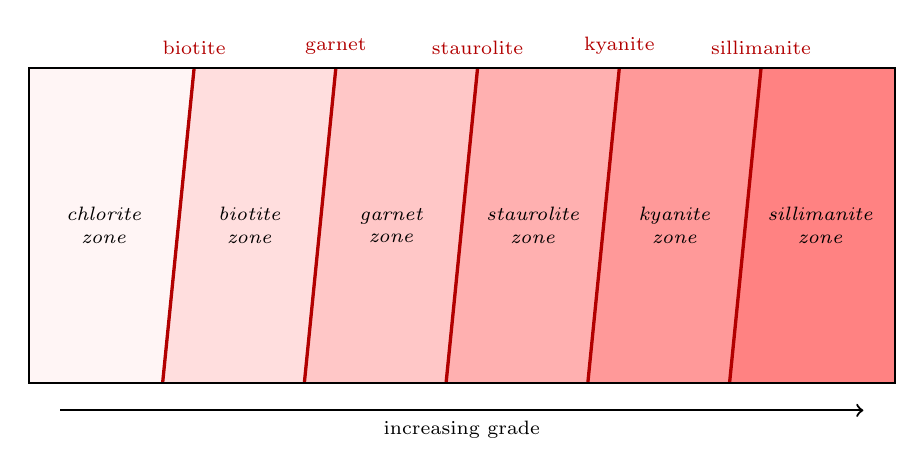
\begin{tikzpicture}[x=1cm, y=1cm]
\def\iso{{0,1.9,3.7,5.5,7.3,9.1,11}}
\foreach \i [evaluate=\i as \op using 4+9*\i] in {0,...,5} {
  \pgfmathsetmacro{\xa}{\iso[\i]}\pgfmathsetmacro{\xb}{\iso[\i+1]}
  \pgfmathsetmacro{\da}{(\i>0)*0.2}\pgfmathsetmacro{\db}{(\i<5)*0.2}
  \fill[red!\op!white] (\xa-\da,0) -- (\xb-\db,0) -- (\xb+\db,4) -- (\xa+\da,4) -- cycle;
}
\foreach \x/\n in {1.9/biotite, 3.7/garnet, 5.5/staurolite, 7.3/kyanite, 9.1/sillimanite} {
  \draw[very thick, red!70!black] (\x-0.2,0) -- (\x+0.2,4);
  \node[font=\scriptsize, red!70!black, anchor=south] at (\x+0.2,4.05) {\n};
}
\draw[thick] (0,0) rectangle (11,4);
\foreach \x/\z in {0.95/chlorite, 2.8/biotite, 4.6/garnet, 6.4/staurolite, 8.2/kyanite, 10.05/sillimanite}
  \node[font=\scriptsize\itshape, align=center] at (\x,2) {\z\\zone};
\draw[->, thick] (0.4,-0.35) -- node[below, font=\scriptsize] {increasing grade} (10.6,-0.35);
\end{tikzpicture}
\par\smallskip{\small \omterm{def:b2:pt-paths:barrovian}{Barrovian zones} on a map, schematic. Each isograd (red line, named
above the map) is the line where its index mineral first appears; grade, and the depth of
the shading, rise to the right. Each zone is named after the mineral that appears at its
low-grade boundary.}
\end{omfigure}
% ledger: iugs:barrow

Isograds are mapped from mineral appearances, and only become conditions of pressure and
temperature once the reactions behind them are known. To go further, one needs to measure
temperature and pressure in a single rock.

\section{Thermometers and barometers}\label{sec:b2:pt-paths:thermobarometry}

\begin{definition}[Geothermometer; geobarometer; exchange reaction; net-transfer reaction]\label{def:b2:pt-paths:thermobarometry}
A \emph{geothermometer}\index{geothermometer} (\emph{geobarometer}\index{geobarometer}) is
an equilibrium among minerals whose position depends mainly on temperature (pressure), so
that the compositions of the minerals give the temperature (pressure) of their last
equilibrium. An \emph{exchange reaction}\index{exchange reaction} swaps two elements
between two minerals, such as iron and magnesium between garnet and biotite, without
creating or destroying either mineral. A \emph{net-transfer reaction}\index{net-transfer
reaction} makes some minerals at the expense of others.
\end{definition}

The most widely used thermometer of \omterm{def:b2:metamorphic-facies:protoliths}{metapelites} is the exchange of iron and magnesium
between garnet and biotite,
\[
\ce{Fe3Al2Si3O12 + KMg3AlSi3O10(OH)2 <=> Mg3Al2Si3O12 + KFe3AlSi3O10(OH)2},
\]
almandine plus phlogopite giving pyrope plus annite. Let $X_{\text{Mg}}$ and $X_{\text{Fe}}$
be the fractions of the sites filled by magnesium and iron in each mineral, and
\[
K_D = \frac{(X_{\text{Mg}}/X_{\text{Fe}})_{\text{garnet}}}{(X_{\text{Mg}}/X_{\text{Fe}})_{\text{biotite}}}.
\]
% ledger: h97:fs-reaction

\begin{proposition}[An exchange equilibrium]\label{prop:b2:pt-paths:exchange}
If garnet and biotite are ideal solutions and $\Delta_r H$, $\Delta_r S$ and $\Delta_r V$ of
the reaction above are constant, then at equilibrium
\[
3RT\ln K_D = -(\Delta_r H + P\,\Delta_r V) + T\,\Delta_r S,
\qquad\text{so}\qquad
T = \frac{\Delta_r H + P\,\Delta_r V}{\Delta_r S - 3R\ln K_D}.
\]
\end{proposition}

\begin{proof}
Each mineral has three sites for iron or magnesium. In an ideal solution the activity of
an end member is the product of the fractions of its sites it fills: $a_{\text{pyrope}} =
X_{\text{Mg}}^3$ in garnet, and so on. The equilibrium constant is therefore
\[
K = \frac{a_{\text{pyrope}}\,a_{\text{annite}}}{a_{\text{almandine}}\,a_{\text{phlogopite}}}
= \frac{X_{\text{Mg,grt}}^3\,X_{\text{Fe,bt}}^3}{X_{\text{Fe,grt}}^3\,X_{\text{Mg,bt}}^3} = K_D^3 .
\]
At equilibrium $\Delta_r G^\circ(T, P) + RT\ln K = 0$, with $\Delta_r G^\circ = \Delta_r H -
T\,\Delta_r S + P\,\Delta_r V$ (the 1 of $P - 1$ neglected), which gives the first equation;
solving it for $T$ gives the second.
\end{proof}

The constants come from experiments in which synthetic garnet and biotite exchanged iron
and magnesium at known temperature and \qty{2.07}{kbar}. Twelve such brackets, from 550 to
\qty{800}{\celsius}, plotted as $\ln K_D$ against $1/T$, fall close to a line (the figure
below); fitted by least squares with $\Delta_r V = \qty{0.311}{J.bar^{-1}}$, they give
$\Delta_r H = \qty{52630}{J}$ and $\Delta_r S = \qty{20.19}{J.K^{-1}}$, the values of
published recalculations of the same data. At higher temperature the ratio $K_D$ rises
towards 1: garnet takes a larger share of the magnesium.
% ledger: h97:fs-data, h97:ideal, h97:fs-reaction

\begin{omfigure}
\centering
\begin{tikzpicture}
\begin{axis}[omrecord, width=0.62\linewidth, height=5.2cm,
  xmin=0.9, xmax=1.25, ymin=-1.9, ymax=-1.1,
  xlabel={$1000/T$ (\unit{K^{-1}})}, ylabel={$\ln K_D$},
  tick label style={font=\scriptsize}, label style={font=\small},
  x tick label style={/pgf/number format/.cd, fixed, precision=2}]
\addplot[only marks, mark=*, mark size=1.6pt, blue!70!black]
  table[x expr={1000/(\thisrow{T_C}+273.15)}, y=lnKD] {figdata/out/bachelor-2-ptpaths-fs.dat};
\addplot[thick, red!75!black, domain=0.9:1.25, samples=2] {(-52630-2070*0.311)/(3*8.31441)*x/1000 + 20.19/(3*8.31441)};
\end{axis}
\end{tikzpicture}
\par\smallskip{\small Garnet--biotite exchange: the twelve experimental brackets at
\qty{2.07}{kbar} (blue, as tabulated by Holdaway and co-authors, 1997) and the line of
the proposition with the fitted $\Delta_r H$ and $\Delta_r S$ (red).}
\end{omfigure}
% ledger: h97:fs-data, h97:ideal

For $K_D = 0.18$ at \qty{5}{kbar}, $T = (52630 + 0.311\times5000)/(20.19 - 3\times8.314
\times\ln 0.18) = 54185/62.96 = \qty{861}{K}$, or \qty{587}{\celsius}. One more kilobar
adds $0.311\times1000/62.96 = \qty{4.9}{K}$: the reaction swaps ions of the same charge
between sites of nearly the same size, its volume change is small, and pressure barely
matters. That is what makes a thermometer.

A barometer needs the opposite: a reaction with a large volume change. The \omterm{def:b2:pt-paths:thermobarometry}{net-transfer
reaction}
\[
\ce{3 CaAl2Si2O8 <=> Ca3Al2Si3O12 + 2 Al2SiO5 + SiO2},
\]
anorthite giving grossular, kyanite and quartz, packs the atoms of three feldspars into
denser minerals: $\Delta_r V = \qty{-6.21}{J.bar^{-1}}$, twenty times that of the exchange.
Its end-member equilibrium, reversed in experiments at 900 to \qty{1250}{\celsius} and 19
to \qty{28}{kbar}, runs along
\[
P_0 = 22.80\,T - 1093 \qquad (P_0 \text{ in bar}, T \text{ in } \unit{\celsius}).
\]
In a rock, grossular is a small part of the garnet and anorthite a part of the
plagioclase. With ideal activities, $a_{\text{grossular}} = X_{\text{Ca,grt}}^3$ and
$a_{\text{anorthite}} = X_{\text{an}}$, the condition $\Delta_r G^\circ + RT\ln K = 0$
written at $P$ and at $P_0$ gives
\[
P = P_0 + \frac{RT}{6.21}\,\ln\frac{X_{\text{Ca,grt}}^3}{X_{\text{an}}^3}
\qquad (T \text{ in kelvin in the second term}).
\]
This \omterm{def:b2:pt-paths:thermobarometry}{geobarometer}, named GASP after the four minerals (garnet, aluminosilicate, silica,
plagioclase), serves wherever a \omterm{def:b2:metamorphic-facies:protoliths}{metapelite} holds all four.
% ledger: kn88:gasp, rh95:gb-gasp

\begin{method}[Temperature and pressure of one rock]\label{met:b2:pt-paths:intersection}
(1) Measure, in minerals that grew together, the compositions the thermometer and the
barometer need. (2) Guess a pressure and compute the temperature with the thermometer.
(3) At that temperature, compute the pressure with the barometer. (4) Repeat (2) and (3)
until neither changes; two or three rounds suffice, since each equation depends weakly on
the variable the other one fixes. Graphically, the answer is where the line of the
thermometer crosses the line of the barometer. (5) Propagate the uncertainties: for
independent errors, $\sigma_T^2 = (\partial T/\partial\ln K_D)^2\sigma_{\ln K_D}^2 +
(\partial T/\partial P)^2\sigma_P^2$, and similarly for $P$.
\end{method}

\begin{omfigure}
\centering
\begin{tikzpicture}
\begin{axis}[omrecord, width=0.78\linewidth, height=6.4cm,
  xmin=400, xmax=800, ymin=0, ymax=12, xlabel={$T$ (\unit{\celsius})}, ylabel={$P$ (\unit{kbar})},
  tick label style={font=\scriptsize}, label style={font=\small}, clip=false]
\addplot[thick, red!75!black] table[x=kd12, y=P_kbar] {figdata/out/bachelor-2-ptpaths-gb.dat};
\addplot[thick, red!75!black] table[x=kd15, y=P_kbar] {figdata/out/bachelor-2-ptpaths-gb.dat};
\addplot[thick, red!75!black] table[x=kd18, y=P_kbar] {figdata/out/bachelor-2-ptpaths-gb.dat};
\addplot[thick, red!75!black] table[x=kd21, y=P_kbar] {figdata/out/bachelor-2-ptpaths-gb.dat};
\addplot[thick, red!75!black] table[x=kd24, y=P_kbar] {figdata/out/bachelor-2-ptpaths-gb.dat};
\addplot[thick, blue!70!black] table[x=T_C, y=r15] {figdata/out/bachelor-2-ptpaths-gasp.dat};
\addplot[thick, blue!70!black] table[x=T_C, y=r20] {figdata/out/bachelor-2-ptpaths-gasp.dat};
\addplot[thick, blue!70!black] table[x=T_C, y=r25] {figdata/out/bachelor-2-ptpaths-gasp.dat};
\addplot[thick, blue!70!black] table[x=T_C, y=r30] {figdata/out/bachelor-2-ptpaths-gasp.dat};
\node[font=\tiny, red!75!black, anchor=west] at (axis cs:452,0.5) {0.12};
\node[font=\tiny, red!75!black, anchor=west] at (axis cs:511,0.5) {0.15};
\node[font=\tiny, red!75!black, anchor=west] at (axis cs:568,0.5) {0.18};
\node[font=\tiny, red!75!black, anchor=west] at (axis cs:622,0.5) {0.21};
\node[font=\tiny, red!75!black, anchor=west] at (axis cs:675,0.5) {0.24};
\node[font=\tiny, blue!70!black, anchor=west] at (axis cs:802,8.97) {0.15};
\node[font=\tiny, blue!70!black, anchor=west] at (axis cs:802,10.21) {0.20};
\node[font=\tiny, blue!70!black, anchor=west] at (axis cs:802,11.17) {0.25};
\node[font=\tiny, blue!70!black, anchor=west] at (axis cs:802,11.96) {0.30};
\end{axis}
\end{tikzpicture}
\par\smallskip{\small Garnet--biotite isotherms (red, steep, labelled with $K_D$) and GASP
isobars (blue, labelled at the right with the ratio $X_{\text{Ca}}/X_{\text{an}}$ of
grossular in garnet to anorthite in plagioclase), from the calibrations of this section. A rock that holds both pairs lies
where its two lines cross.}
\end{omfigure}
% ledger: h97:ideal, h97:fs-reaction, kn88:gasp

The thermometer lines are nearly vertical, the barometer lines inclined: they cross at a
wide angle, which keeps the intersection precise. Ideal mixing is the main simplification
of this chapter. Real garnets hold calcium and manganese, real biotites aluminium,
titanium and ferric iron, and calibrations that correct for them shift temperatures by
tens of degrees (in one well-studied region, \qty{574}{\celsius} instead of
\qty{530}{\celsius}); the best ones claim an uncertainty of about \qty{25}{\celsius}.
% ledger: h97:ideal, h97:corrections

\section{Pressure--temperature paths}\label{sec:b2:pt-paths:paths}

A rock does not reach its highest pressure and highest temperature at the same moment.
It is buried and heated, then brought back up and cooled, and its minerals react all
along.

\begin{definition}[P--T path; prograde and retrograde paths; peak metamorphic conditions]\label{def:b2:pt-paths:paths}
The \emph{P--T path}\index{P--T path} of a rock is the sequence of pressures and
temperatures it passed through during a metamorphic event. Its \emph{prograde
path}\index{prograde path} is the part along which temperature rises, its \emph{retrograde
path}\index{retrograde path} the part along which it falls. The \emph{peak metamorphic
conditions}\index{peak metamorphic conditions} are the pressure and temperature at the
highest temperature of the path, the thermal peak; the pressure peak, or baric peak, need
not coincide with it.
\end{definition}
% ledger: scmr:ptt

A path is \emph{clockwise} when, drawn with temperature to the right and pressure upwards,
the thermal peak comes after the baric peak, during decompression; it is
\emph{anticlockwise} when the thermal peak is reached while pressure still rises. Which
sense a rock follows depends on how heat reached it, and the simplest case can be
computed.
% ledger: scmr:ptt

Imagine a crust \qty{35}{km} thick, at steady state, with a heat production of
\qty{1.0}{\micro W.m^{-3}}, a heat flow of \qty{25}{mW.m^{-2}} from below, a conductivity
of \qty{2.5}{W.m^{-1}.K^{-1}} and a diffusivity of \qty{1e-6}{m^2.s^{-1}}, the last three
within the ranges measured on rocks. Its surface heat flow is \qty{60}{mW.m^{-2}} and its Moho lies at
\qty{595}{\celsius}. A collision stacks a second copy of this crust on top of it, quickly
compared with the time heat needs to move: the rocks of the lower sheet keep their
temperatures but sit \qty{35}{km} deeper, so that the geotherm becomes a sawtooth, with
rocks at \qty{0}{\celsius} at \qty{35}{km} beneath hot rocks of the upper sheet. The crust is
now \qty{70}{km} thick and holds twice the heat-producing rock. Thirty million years after
the stacking, erosion begins and removes \qty{35}{km} in 70 million years
(\qty{0.5}{mm.yr^{-1}}).
% ledger: delaney:conductivity, roy:granitic-k, vila:heat-production, prem:moho-average, et84:ptt

\begin{proposition}[Time scale of thermal relaxation]\label{prop:b2:pt-paths:relaxation}
In a layer of thickness $L$ whose two faces are held at fixed temperature, a temperature
disturbance of the form $\sin(\pi z/L)$ decays as $e^{-t/\tau}$, with
\[
\tau = \frac{L^2}{\pi^2\kappa}.
\]
\end{proposition}

\begin{proof}
Write $\theta(z, t) = f(t)\sin(\pi z/L)$, which vanishes at $z = 0$ and $z = L$. The heat
equation $\partial\theta/\partial t = \kappa\,\partial^2\theta/\partial z^2$ gives
$f'\sin(\pi z/L) = -\kappa(\pi/L)^2 f\sin(\pi z/L)$, so $f' = -f/\tau$ with $\tau =
L^2/(\pi^2\kappa)$, and $f = f(0)\,e^{-t/\tau}$.
\end{proof}

The sawtooth has a wavelength of the order of the thickness of one sheet: with $L =
\qty{35}{km}$, $\tau = \qty{3.9}{Myr}$, and the cold wedge at \qty{35}{km} is erased within
ten million years. The whole thickened crust, $L = \qty{70}{km}$, relaxes on $\tau =
\qty{16}{Myr}$, so that heating continues for tens of millions of years, towards the much
hotter geotherm that a crust twice as thick and with twice the heat-producing rock
supports. The figure
below shows the computed geotherms.
% ledger: delaney:conductivity

\begin{omfigure}
\centering
\begin{tikzpicture}
\begin{axis}[omrecord, width=0.62\linewidth, height=6.6cm,
  xmin=0, xmax=1000, ymin=0, ymax=80, y dir=reverse,
  xlabel={$T$ (\unit{\celsius})}, ylabel={depth (\unit{km})},
  legend style={font=\scriptsize, at={(0.02,0.02)}, anchor=south west},
  tick label style={font=\scriptsize}, label style={font=\small}]
\addplot[thick, black] table[x=t0, y=z_km] {figdata/out/bachelor-2-ptpaths-geo.dat};
\addlegendentry{\qty{0}{Myr}}
\addplot[thick, blue!70!black] table[x=t10, y=z_km] {figdata/out/bachelor-2-ptpaths-geo.dat};
\addlegendentry{\qty{10}{Myr}}
\addplot[thick, orange!85!black] table[x=t30, y=z_km] {figdata/out/bachelor-2-ptpaths-geo.dat};
\addlegendentry{\qty{30}{Myr}}
\addplot[thick, red!75!black] table[x=t60, y=z_km] {figdata/out/bachelor-2-ptpaths-geo.dat};
\addlegendentry{\qty{60}{Myr}}
\end{axis}
\end{tikzpicture}
\par\smallskip{\small Geotherms after doubling a \qty{35}{km} crust by stacking, computed
with the heat equation (depths below the surface of the moment; erosion starts at
\qty{30}{Myr}). Black: the sawtooth just after stacking. The base of the thickened crust,
at \qty{595}{\celsius} at first, passes \qty{900}{\celsius} after 60 million years.}
\end{omfigure}
% ledger: et84:ptt

Follow the rock that was at the surface before the stacking and lies at \qty{35}{km} just
after it, under \qty{9.6}{kbar}. In five million years it warms from 0 to
\qty{395}{\celsius} without moving; by the start of erosion it has reached
\qty{558}{\celsius}. Erosion then brings it up, but heat keeps arriving faster than it
escapes: the rock is still warming when it has risen \qty{6}{km}, and reaches its thermal
peak, \qty{593}{\celsius} at \qty{7.8}{kbar}, 43 million years after the stacking. Only
then does it cool, through \qty{405}{\celsius} at \qty{13}{km} depth and
\qty{74}{Myr}, on its way to the surface. The path (the figure below) is clockwise. It also
stays within \qty{50}{\celsius} of its peak temperature for thirty million years, about a
third of its whole journey, as England and Thompson found in 1984 for most geologically
plausible cases: a rock spends a long time close to its peak, and the minerals it keeps
mostly record that stage.
% ledger: et84:ptt

\begin{omfigure}
\centering
\begin{tikzpicture}
\begin{axis}[omrecord, width=0.78\linewidth, height=6.2cm,
  xmin=0, xmax=800, ymin=0, ymax=11, xlabel={$T$ (\unit{\celsius})}, ylabel={$P$ (\unit{kbar})},
  tick label style={font=\scriptsize}, label style={font=\small}]
\addplot[thick, gray, densely dashed, restrict x to domain=0:504] table[x=T_C, y=P_kbar] {figdata/out/bachelor-2-facies-hm93-kyand.dat};
\addplot[thick, gray, densely dashed] table[x=T_C, y=P_kbar] {figdata/out/bachelor-2-facies-hm93-kysil.dat};
\addplot[thick, gray, densely dashed] table[x=T_C, y=P_kbar] {figdata/out/bachelor-2-facies-hm93-andsil.dat};
\addplot[very thick, red!75!black, postaction={decorate}, decoration={markings,
  mark=at position 0.2 with {\arrow{Stealth[length=2.5mm]}},
  mark=at position 0.52 with {\arrow{Stealth[length=2.5mm]}},
  mark=at position 0.8 with {\arrow{Stealth[length=2.5mm]}}}] table[x=T_C, y=P_kbar] {figdata/out/bachelor-2-ptpaths-path.dat};
\node[font=\scriptsize\bfseries, gray] at (axis cs:330,6.5) {kyanite};
\node[font=\scriptsize\bfseries, gray] at (axis cs:520,1.0) {andalusite};
\node[font=\scriptsize\bfseries, gray] at (axis cs:740,4.0) {sillimanite};
\node[font=\scriptsize, red!75!black, anchor=south] at (axis cs:200,9.7) {heating at depth};
\node[font=\scriptsize, red!75!black, anchor=west] at (axis cs:603,8.9) {thermal peak};
\node[font=\scriptsize, red!75!black, anchor=west] at (axis cs:110,2.7) {cooling ascent};
\end{axis}
\end{tikzpicture}
\par\smallskip{\small \omterm{def:b2:pt-paths:paths}{P--T path} of the rock that lies at \qty{35}{km} just after the
stacking (red, sampled every two million years), computed with the model of the geotherms above,
over the experimental \ce{Al2SiO5} diagram of \cref{ch:b2:metamorphic-facies} (grey). The
pressure peak comes first, the thermal peak during decompression: a clockwise path, which
never leaves the kyanite field.}
\end{omfigure}
% ledger: et84:ptt, hm93:table11

The model also shows why some paths turn the other way. Thickening alone heats a rock
only after it has been buried, so its thermal peak comes during \omterm{def:b2:pt-paths:exhumation}{exhumation}. A rock whose
temperature rises while it is still being buried needs heat from elsewhere, such as \omterm{def:b2:magma-emplacement:magma}{magma}
rising into the crust above or beside it, and follows an anticlockwise path. And in the
thickened crust the base heats far above its initial temperature: England and Thompson
concluded that considerable melting of the crust is a likely consequence of thickening,
the subject of \cref{ch:b2:crustal-melting}.
% ledger: et84:ptt, scmr:ptt

\section{Adding time}\label{sec:b2:pt-paths:time}

\begin{definition}[P--T--t path]\label{def:b2:pt-paths:ptt}
The \emph{P--T--t path}\index{P--T--t path} of a rock is its \omterm{def:b2:pt-paths:paths}{P--T path} with the time at
which each point was reached.
\end{definition}
% ledger: scmr:ptt

Time comes from radiometric dating. A mineral that grew during the event and has kept
its daughter isotopes since, such as a zone of garnet dated by the
samarium--neodymium method, dates its own growth, and its
composition gives the pressure and temperature of that moment. A mineral that grew
earlier, at higher temperature, gives instead a cooling age: the time at which the rock
cooled through the closure temperature of that mineral and isotope system (Year 1
volume). For argon in a muscovite grain of \qty{100}{\micro m} radius, cooling at
\qty{10}{\celsius} per million years, the closure temperature is \qty{405}{\celsius} at
\qty{5}{kbar} and \qty{425}{\celsius} at \qty{10}{kbar}.
% ledger: h09:muscovite

\begin{definition}[Exhumation; exhumation rate]\label{def:b2:pt-paths:exhumation}
\emph{Exhumation}\index{exhumation} is the movement of a rock towards the Earth's surface,
by removal of the rocks above it. The \emph{exhumation rate}\index{exhumation rate} is the
rate of decrease of its depth.
\end{definition}

\begin{proposition}[Rates from two dated points]\label{prop:b2:pt-paths:rates}
If a rock was at temperature $T_1$ and depth $z_1$ at time $t_1$ and at $T_2$, $z_2$ at a
later time $t_2$ (ages counted back from today, $t_1 > t_2$), its mean cooling and
\omterm{def:b2:pt-paths:exhumation}{exhumation rates} over the interval are
\[
\frac{T_1 - T_2}{t_1 - t_2}
\qquad\text{and}\qquad
\frac{z_1 - z_2}{t_1 - t_2},
\]
and their uncertainties, for independent errors on the two ages, follow from
$\sigma_{t_1 - t_2}^2 = \sigma_{t_1}^2 + \sigma_{t_2}^2$.
\end{proposition}

\begin{proof}
A mean rate is a difference divided by the elapsed time $t_1 - t_2$; the variance of a
difference of independent quantities is the sum of their variances.
\end{proof}

The depth at which a cooling age was set is rarely measured: it is estimated from the
geotherm of the time, which is why \omterm{def:b2:pt-paths:exhumation}{exhumation rates} are less certain than cooling rates.
A pressure, where a \omterm{def:b2:metamorphic-facies:assemblage}{mineral assemblage} gives one, fixes the depth directly, as
$z = P/(\bar\rho g)$ with $\bar\rho$ the mean density of the rocks above.

\section{Metamorphic series and paired belts}\label{sec:b2:pt-paths:series}

\begin{definition}[Metamorphic series; paired metamorphic belts]\label{def:b2:pt-paths:series}
A \emph{metamorphic series}\index{metamorphic series} (or facies series) is a sequence of
\omterm{def:b2:metamorphic-facies:facies}{metamorphic facies} developed under the same range of ratios of pressure to temperature,
and therefore occupying a radial sector of the pressure--temperature plane.
\emph{Paired metamorphic belts}\index{paired metamorphic belts} are two parallel belts of
the same age, one of high-pressure series and one of low-pressure series.
\end{definition}
% ledger: scmr:ptt, wallis24:paired

Three series are commonly distinguished. A high ratio of pressure to temperature, along a
cold gradient, leads from the zeolite facies to the blueschists and eclogites: the series
of subduction zones. An intermediate ratio leads through the greenschist, amphibolite and
granulite facies, with kyanite then sillimanite in \omterm{def:b2:metamorphic-facies:protoliths}{metapelites}: the Barrovian series. A low
ratio, along hot gradients such as those near intrusions, produces andalusite then
sillimanite: the low-pressure or Buchan series. The figure below draws three gradients
across the aluminosilicate diagram.
% ledger: scmr:ptt, scmr:facies, iugs:barrow, fub:paired

\begin{omfigure}
\centering
\begin{tikzpicture}
\begin{axis}[omrecord, width=0.78\linewidth, height=6.2cm,
  xmin=0, xmax=900, ymin=0, ymax=12, xlabel={$T$ (\unit{\celsius})}, ylabel={$P$ (\unit{kbar})},
  tick label style={font=\scriptsize}, label style={font=\small}]
\addplot[thick, gray, densely dashed, restrict x to domain=0:504] table[x=T_C, y=P_kbar] {figdata/out/bachelor-2-facies-hm93-kyand.dat};
\addplot[thick, gray, densely dashed] table[x=T_C, y=P_kbar] {figdata/out/bachelor-2-facies-hm93-kysil.dat};
\addplot[thick, gray, densely dashed] table[x=T_C, y=P_kbar] {figdata/out/bachelor-2-facies-hm93-andsil.dat};
\addplot[very thick, blue!70!black] table[x=T_C, y=g10] {figdata/out/bachelor-2-ptpaths-series.dat};
\addplot[very thick, green!45!black] table[x=T_C, y=g25] {figdata/out/bachelor-2-ptpaths-series.dat};
\addplot[very thick, orange!85!black] table[x=T_C, y=g60] {figdata/out/bachelor-2-ptpaths-series.dat};
\node[font=\scriptsize, blue!70!black, rotate=52, anchor=south] at (axis cs:330,8.5) {\qty{10}{\celsius\per\km}};
\node[font=\scriptsize, green!45!black, rotate=28, anchor=south] at (axis cs:640,7.0) {\qty{25}{\celsius\per\km}};
\node[font=\scriptsize, orange!85!black, rotate=12, anchor=south] at (axis cs:800,3.65) {\qty{60}{\celsius\per\km}};
\node[font=\scriptsize\bfseries, gray] at (axis cs:120,5.5) {kyanite};
\node[font=\scriptsize\bfseries, gray] at (axis cs:470,1.1) {andalusite};
\node[font=\scriptsize\bfseries, gray] at (axis cs:800,1.6) {sillimanite};
\end{axis}
\end{tikzpicture}
\par\smallskip{\small Three geothermal gradients from a surface at \qty{10}{\celsius},
converted to pressure with a mean density of \qty{2800}{kg.m^{-3}}, over the experimental
\ce{Al2SiO5} diagram (grey). The cold gradient stays in the kyanite field, the
intermediate one passes from kyanite to sillimanite, the hot one crosses the andalusite
field before it reaches sillimanite.}
\end{omfigure}
% ledger: hm93:table11

The idea of the series came from Japan, where Akiho Miyashiro defined them in 1961. In
the southwest of the country the Sanbagawa belt, of high-pressure, low-temperature
\omterm{def:b2:metamorphic-facies:metamorphism}{metamorphism}, runs for more than \qty{800}{km} beside the Ryoke belt, of high-temperature,
low-pressure \omterm{def:b2:metamorphic-facies:metamorphism}{metamorphism}, the two separated by a major fault: the classic pair. The
Sanbagawa belt is an ancient subduction zone, the Ryoke belt the volcanic arc above it. A
subduction zone thus makes both series at once, cold rocks dragged down by the sinking
plate, hot ones heated in the arc; paired belts of the same kind are known around the
Pacific.
% ledger: wallis24:paired, koguchi17:paired, fub:paired, scmr:ptt

\section{Ultrahigh pressure and exhumation}\label{sec:b2:pt-paths:uhp}

In 1984 a quartzite was described from the Dora Maira massif of the Western
Alps whose garnets, up to \qty{25}{cm} across and almost pure pyrope, enclose grains of
coesite, the dense polymorph of silica, partly turned back to quartz; the expansion
during that inversion cracked the host garnet radially around each grain. The coesite and
its companions imply at least \qty{28}{kbar} at about \qty{700}{\celsius}: rocks of the
upper continental crust, once sediments, had gone down to \qty{90}{km} or more and come
back.
% ledger: chopin84:coesite

\begin{definition}[Ultrahigh-pressure metamorphism]\label{def:b2:pt-paths:uhp}
\emph{Ultrahigh-pressure metamorphism}\index{ultrahigh-pressure metamorphism} is
\omterm{def:b2:metamorphic-facies:metamorphism}{metamorphism} of crustal rocks at pressures high enough for coesite, or diamond, to grow.
\end{definition}

\begin{omfigure}
\centering
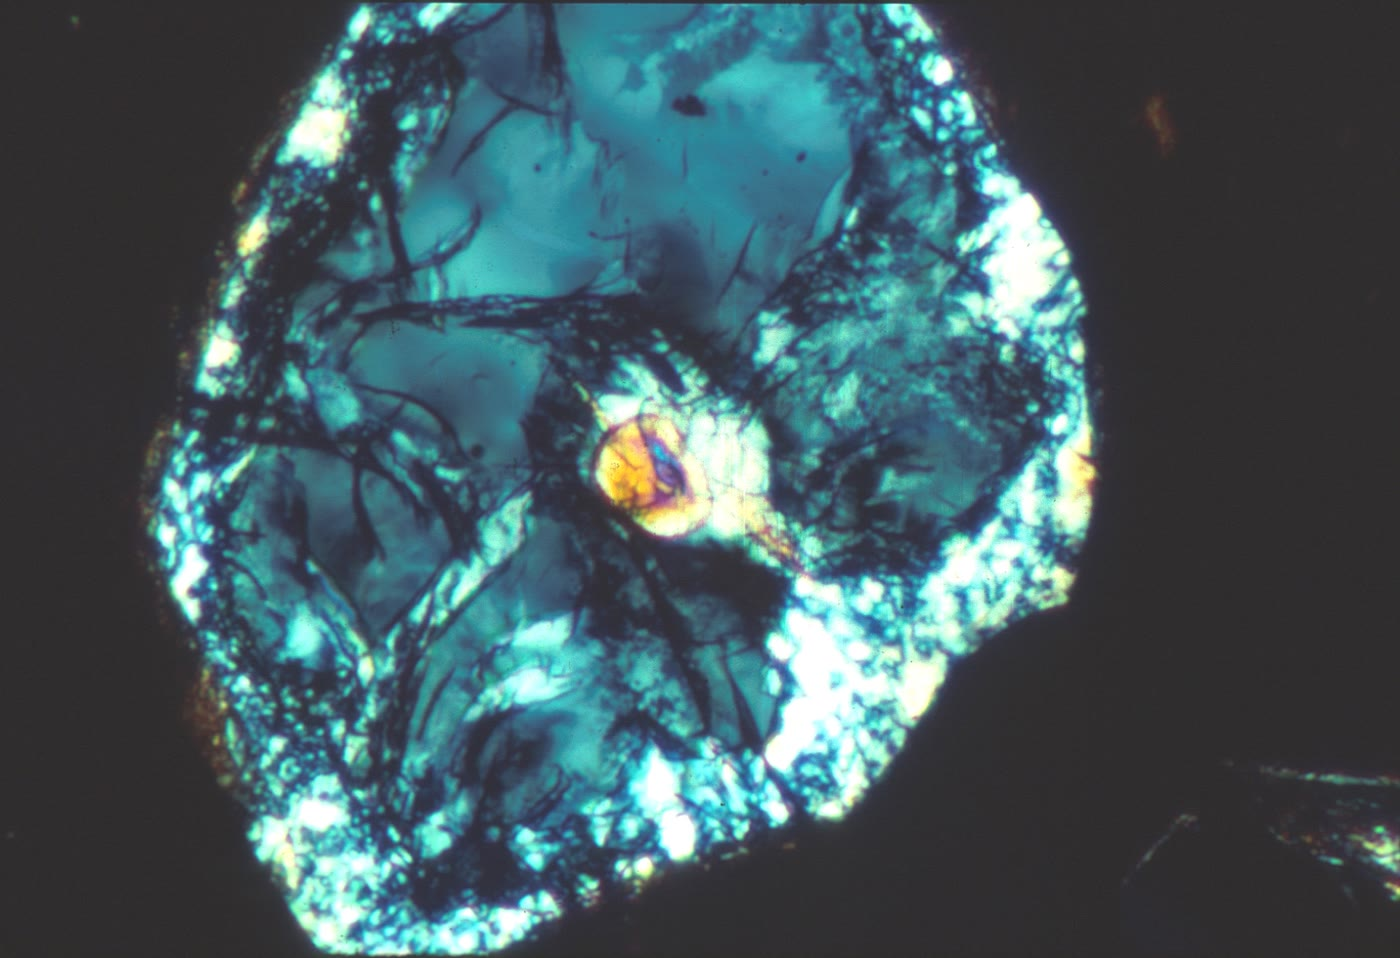
\includegraphics[width=0.62\linewidth]{images/book4/b2-11-coesite.jpg}
\par\smallskip{\small Coesite in an eclogite, about \qty{1}{mm} across, in a thin section
between crossed polarisers: the large central grain is coesite, the rim of small bright grains is
quartz that grew from it as the pressure fell; the small coloured grain in the centre is a
pyroxene inclusion. Photograph J.\,R. Smyth, CC BY-SA 1.0.}
\end{omfigure}

Six years later, diamonds averaging \qty{12}{\micro m} were found in gneisses, schists and
garnet--pyroxene rocks of the Kokchetav massif of northern Kazakhstan, enclosed in garnet
and zircon, which shielded them from turning into graphite: they grew at \qty{40}{kbar}
or more and above 900 to \qty{1000}{\celsius}. Continental crust, light as it is, can be
dragged more than a hundred kilometres down.
% ledger: ss90:diamond

How it comes back is told by its clocks. In the deepest subducted rocks of the Alps,
titanite dated at successive stages shows that a calc-silicate rock reached about
\qty{3.5}{GPa} at $35.1 \pm \qty{0.9}{Ma}$, was at $1 \pm \qty{0.15}{GPa}$ at $32.9 \pm
\qty{0.9}{Ma}$, and near 0.4 to \qty{0.5}{GPa} at $31.8 \pm \qty{0.5}{Ma}$. The mean
\omterm{def:b2:pt-paths:exhumation}{exhumation rates}, 3.4 then \qty{1.6}{cm.yr^{-1}}, match the speeds of plates: the rocks
came back about as fast as they went down, much faster than erosion could have unroofed
them. The authors invoke buoyancy, the light crust rising through the denser mantle, and
normal faulting, which thins the rocks above.
% ledger: rh01:exhumation

\section{Ocean-floor metamorphism}\label{sec:b2:pt-paths:ocean-floor}

\begin{definition}[Ocean-floor metamorphism; serpentinisation]\label{def:b2:pt-paths:ocean-floor}
\emph{Ocean-floor metamorphism}\index{ocean-floor metamorphism} is the regional
\omterm{def:b2:metamorphic-facies:metamorphism}{metamorphism} of the oceanic lithosphere near spreading centres, by hot aqueous fluids
circulating under steep geothermal gradients; recrystallisation is generally incomplete
and temperature typically increases with depth. \emph{Serpentinisation}\index{serpentinisation}
is the hydration of olivine-rich rocks into serpentine.
\end{definition}
% ledger: scmr:types

Seawater drawn into the young crust near a ridge axis heats up, reacts with the rocks and
rises again. The basalts it passes through recrystallise, incompletely, into hydrous
minerals, over a wide range of temperatures. Where the water reaches \omterm{def:b2:mantle-melting:peridotites}{peridotite}, as on
the slow ridges where mantle rock comes up to the sea floor and feeds springs such as
those of the Lost City field (Year 1 volume), olivine takes up water:
\[
\ce{2 Mg2SiO4 + 3 H2O -> Mg3Si2O5(OH)4 + Mg(OH)2},
\]
forsterite giving serpentine and brucite. The molar volumes, 43.65 for forsterite, 107.50
for serpentine and \qty{24.63}{cm^3.mol^{-1}} for brucite, show what this does to the rock:
\qty{87.30}{cm^3} of olivine become \qty{132.13}{cm^3} of solids, \qty{51}{\percent}
more, and the density falls from 3.22 to \qty{2.54}{g.cm^{-3}}. The rock swells and
lightens, and the water it has bound goes down with it when the plate is subducted.
% ledger: scmr:types, rh95:serpentine, kelley:lost-city, dick:ultraslow

\begin{inthelab}[Reading a garnet]
To read a \omterm{def:b2:pt-paths:paths}{P--T path}, a petrologist first cuts a thin section through the centre of a
garnet, since a section off-centre misses the core. Under the microscope the inclusions
are mapped: small grains of quartz, biotite, plagioclase or kyanite trapped as the garnet
grew, sometimes aligned in trails that preserve an older foliation of the rock. An electron
microprobe then measures the composition along a line from core to rim, and a map of
magnesium, iron, calcium and manganese shows the growth zones. Each zone is paired with
the minerals that grew with it: inclusions for the core, the matrix in contact for the
rim. Thermometer and barometer are applied to each pair, and the zones are dated where a
mineral allows it. \Cref{ch:b2:field-lab-methods-2} describes the instruments.
\end{inthelab}

\begin{omfigure}
\centering
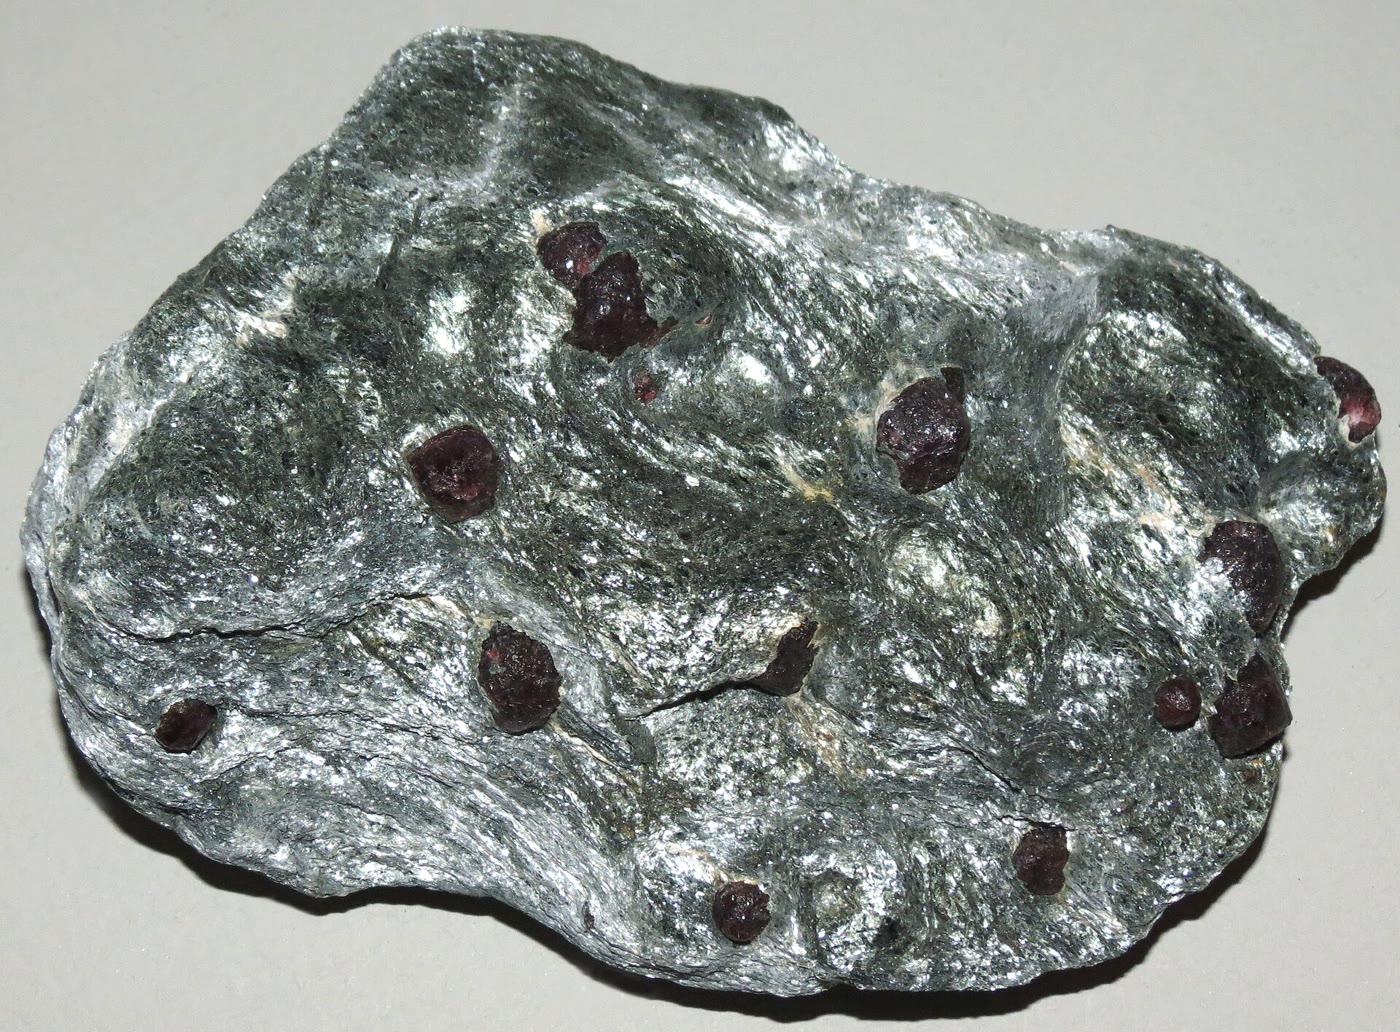
\includegraphics[width=0.62\linewidth]{images/book4/b2-11-garnet-schist.jpg}
\par\smallskip{\small A garnet schist: dark red garnet crystals grown in a foliated
matrix of micas. Each garnet can hold, from core to rim, a
record of the rock's path. Photograph James St.~John, CC BY 2.0.}
\end{omfigure}

\section{Exercises}

\begin{exercise}[$\star$]\label{exo:b2:pt-paths:1}
Six samples of one mudstone formation, collected along a road, hold: (A) chlorite,
muscovite, quartz; (B) biotite, chlorite, muscovite, quartz; (C) garnet, biotite,
muscovite, quartz; (D) staurolite, garnet, biotite, muscovite, quartz; (E) kyanite,
staurolite, biotite, muscovite, quartz; (F) sillimanite, biotite, muscovite, quartz.
(a) In which Barrovian zone does each lie? (b) How many isograds does the road cross, and
which? (c) Why is it not enough to know the isograds to draw the \omterm{def:b2:pt-paths:barrovian}{metamorphic field
gradient}?
\end{exercise}
% ledger: iugs:barrow

\begin{exercise}[$\star$]\label{exo:b2:pt-paths:2}
A garnet has $X_{\text{Mg}} = 0.10$ and $X_{\text{Fe}} = 0.80$, the biotite beside it
$X_{\text{Mg}} = 0.45$ and $X_{\text{Fe}} = 0.50$. (a) Compute $K_D$ and $\ln K_D$.
(b) With the calibration of this chapter, compute the temperature at \qty{5}{kbar} and at
\qty{7}{kbar}. (c) Is the result a temperature or a pressure gauge?
\end{exercise}
% ledger: h97:ideal, h97:fs-reaction

\begin{exercise}[$\star$]\label{exo:b2:pt-paths:3}
A \omterm{def:b2:metamorphic-facies:protoliths}{metapelite} gives \qty{580}{\celsius} and \qty{6.0}{kbar}. (a) Under rocks of mean
density \qty{2800}{kg.m^{-3}} ($g = \qty{9.81}{m.s^{-2}}$), how deep was it? (b) What
temperature gradient does that imply from \qty{10}{\celsius} at the surface? (c) The
experimental kyanite $=$ sillimanite line passes through \qty{3.67}{kbar} at
\qty{500}{\celsius} and \qty{5.77}{kbar} at \qty{600}{\celsius}: which aluminosilicate
should the rock hold?
\end{exercise}
% ledger: hm93:table11

\begin{exercise}[$\star$]\label{exo:b2:pt-paths:4}
For the \omterm{def:b2:pt-paths:ocean-floor}{serpentinisation} of forsterite written in this chapter: (a) check that the
equation is balanced in mass, with molar masses 140.693 (forsterite), 18.015 (water),
277.112 (serpentine) and \qty{58.320}{g.mol^{-1}} (brucite); (b) compute the change in
volume of the solids; (c) compute the densities of the olivine and of the products.
(d) What does the change do to a serpentinised \omterm{def:b2:mantle-melting:peridotites}{peridotite} beneath the sea floor?
\end{exercise}
% ledger: rh95:serpentine

\begin{exercise}[$\star\star$]\label{exo:b2:pt-paths:5}
Calibrate the thermometer from four of the experiments at \qty{2.07}{kbar}: $\ln K_D =
-1.157$ and $-1.255$ at \qty{799}{\celsius}, $-1.738$ and $-1.826$ at \qty{550}{\celsius}.
(a) Average each pair and find the line $\ln K_D = a/T + b$ through the two means.
(b) Deduce $\Delta_r H$ and $\Delta_r S$, with $\Delta_r V = \qty{0.311}{J.bar^{-1}}$.
(c) Compare the temperatures that your calibration and that of the chapter give at
\qty{5}{kbar} for $K_D = 0.18$, $0.10$ and $0.30$. What do you conclude about
extrapolating a calibration?
\end{exercise}
% ledger: h97:fs-data, h97:ideal

\begin{exercise}[$\star\star$]\label{exo:b2:pt-paths:6}
(a) From the molar volumes at \qty{298}{K} (almandine 115.32, pyrope 113.12, annite
154.30, phlogopite 149.65, grossular 125.28, anorthite 100.79, kyanite 44.15, quartz
\qty{22.69}{cm^3.mol^{-1}}), compute $\Delta_r V$ of the exchange and of the GASP
reaction, and compare with the values the calibrations use, \num{0.311} and
\qty{-6.21}{J.bar^{-1}}. (b) For $K_D = 0.18$, by how many kelvin does an error of
\qty{1}{kbar} shift the temperature? (c) Along the GASP line of a rock with
$X_{\text{Ca}}/X_{\text{an}} = 0.20$, by how many bar does an error of \qty{17}{K} shift
the pressure?
\end{exercise}
% ledger: rh95:gb-gasp, rh95:al2sio5, h97:fs-reaction, kn88:gasp

\begin{exercise}[$\star\star$]\label{exo:b2:pt-paths:7}
At \qty{600}{\celsius}, a garnet has $X_{\text{Ca}} = 0.08$ and the plagioclase beside it
$X_{\text{an}} = 0.30$. (a) Compute the GASP pressure. (b) Redo it with $X_{\text{an}} =
0.35$. (c) How deep was the rock, for a mean density of \qty{2800}{kg.m^{-3}}?
\end{exercise}
% ledger: kn88:gasp

\begin{exercise}[$\star\star$]\label{exo:b2:pt-paths:8}
Use the titanite ages of the deepest subducted rocks of the Alps: about \qty{3.5}{GPa} at
$35.1 \pm \qty{0.9}{Ma}$, \qty{1.0}{GPa} at $32.9 \pm \qty{0.9}{Ma}$, \qty{0.45}{GPa} at
$31.8 \pm \qty{0.5}{Ma}$. (a) With a mean density of \qty{3000}{kg.m^{-3}}, convert the
pressures to depths. (b) Compute the two mean \omterm{def:b2:pt-paths:exhumation}{exhumation rates} and compare with the
published 3.4 and \qty{1.6}{cm.yr^{-1}}. (c) What is the uncertainty of the first time
interval, and what range of rates does it allow? (d) Compare with the erosion rate of
the thickening model, \qty{0.5}{mm.yr^{-1}}.
\end{exercise}
% ledger: rh01:exhumation

\begin{exercise}[$\star\star$]\label{exo:b2:pt-paths:9}
For $K_D = 0.18$ at \qty{5}{kbar}, (a) compute $\partial T/\partial\ln K_D$ and
$\partial T/\partial P$ from the proposition; (b) with $\sigma_{\ln K_D} = 0.05$ (a
\qty{5}{\percent} error on $K_D$) and $\sigma_P = \qty{1}{kbar}$, compute $\sigma_T$.
(c) Which error dominates? Compare with the uncertainty of \qty{25}{\celsius} claimed for
the best calibrations.
\end{exercise}
% ledger: h97:ideal

\begin{exercise}[$\star\star\star$]\label{exo:b2:pt-paths:10}
A garnet rim has $X_{\text{Mg}} = 0.10$, $X_{\text{Fe}} = 0.75$, $X_{\text{Ca}} = 0.07$;
the matrix biotite $X_{\text{Mg}} = 0.42$, $X_{\text{Fe}} = 0.52$; the plagioclase
$X_{\text{an}} = 0.25$. (a) Apply the method of this chapter, starting from \qty{6}{kbar},
until the temperature changes by less than \qty{1}{K}. (b) Which aluminosilicate should
the rock hold (use the experimental line of \cref{exo:b2:pt-paths:3})? (c) Why must the barometer use
the aluminosilicate actually present?
\end{exercise}
% ledger: h97:ideal, kn88:gasp, hm93:table11

\begin{exercise}[$\star\star\star$]\label{exo:b2:pt-paths:11}
With $\kappa = \qty{1e-6}{m^2.s^{-1}}$: (a) compute the relaxation time of the
proposition for $L = \qty{35}{km}$ and for $L = \qty{70}{km}$. (b) The model erodes
\qty{35}{km} in 70 million years; compare that time with the two of (a). (c) Explain,
from these times, why the rock of the model reaches its thermal peak after its pressure
peak. (d) If erosion were ten times faster, what would change in the path?
\end{exercise}
% ledger: delaney:conductivity, et84:ptt

\begin{exercise}[$\star\star\star$]\label{exo:b2:pt-paths:12}
Take a crust \qty{35}{km} thick of density \qty{2800}{kg.m^{-3}} above a mantle of
\qty{3300}{kg.m^{-3}}. (a) At what depth does the pressure reach \qty{28}{kbar}, the
minimum for the Dora Maira coesite? (b) And \qty{40}{kbar}, for the Kokchetav diamonds?
(c) What mean gradient does \qty{700}{\celsius} at the depth of (a) imply, and in which
series does it fall? (d) At \qty{3.4}{cm.yr^{-1}}, how long does the climb from the depth
of (a) to \qty{35}{km} take?
\end{exercise}
% ledger: chopin84:coesite, ss90:diamond, rh01:exhumation

\section{Problem: A garnet's journey}

\begin{problem}[{Weekend problem --- thermobarometry, path and exhumation rate of one
schist}]
\label{pb:b2:pt-paths:1}
A kyanite--garnet--biotite schist holds garnets with a core and a rim. The core encloses
biotite, plagioclase and kyanite; the rim touches the biotite and plagioclase of the
matrix. Around the garnets, some kyanite is replaced by sillimanite, and at the edges of
the garnets some chlorite has grown. The analyses are:
\begin{center}
\small
\begin{tabular}{@{}lccc@{}}
\hline
 & $X_{\text{Mg}}$ & $X_{\text{Fe}}$ & $X_{\text{Ca}}$ or $X_{\text{an}}$\\
\hline
garnet core & 0.080 & 0.760 & 0.050\\
biotite included in the core & 0.40 & 0.58 & ---\\
plagioclase included in the core & --- & --- & 0.25\\
garnet rim & 0.120 & 0.720 & 0.060\\
matrix biotite & 0.46 & 0.53 & ---\\
matrix plagioclase & --- & --- & 0.28\\
\hline
\end{tabular}
\end{center}
Use the garnet--biotite thermometer and the GASP barometer of this chapter (ideal mixing),
$R = \qty{8.314}{J.mol^{-1}.K^{-1}}$, $g = \qty{9.81}{m.s^{-2}}$, a mean density of
\qty{2800}{kg.m^{-3}} above the rock, and round each ratio to four decimals.

\noindent\textbf{Part I --- Temperatures.}
\begin{enumerate}
\item Compute $X_{\text{Mg}}/X_{\text{Fe}}$ in the garnet core and in the included
biotite, then $K_D$ and $\ln K_D$ for the core.
\item Do the same for the rim and the matrix biotite.
\item Compute the temperature of the core at \qty{6}{kbar}.
\item Compute the temperature of the rim at \qty{6}{kbar}.
\item By how many kelvin would an error of \qty{1}{kbar} change these temperatures?
\item Why is the core paired with the included biotite, and the rim with the matrix
biotite?
\end{enumerate}

\noindent\textbf{Part II --- Pressures.}
\begin{enumerate}[resume]
\item Compute the end-member pressure $P_0$ of the GASP reaction at the two temperatures
of questions~3 and~4.
\item Compute the GASP pressure of the core at the temperature of question~3.
\item Compute the GASP pressure of the rim at the temperature of question~4.
\item Recompute the temperature of the rim at the pressure of question~9, then its
pressure at that temperature, and once more the temperature. Give the rim's temperature
and pressure.
\item Do the same once for the core. Why does it change so little?
\item Convert the pressures of the core and the rim into depths.
\item The experimental kyanite $=$ sillimanite line passes through 3.67, 5.77 and
\qty{7.86}{kbar} at 500, 600 and \qty{700}{\celsius}. Which aluminosilicate was stable
when the core grew, and when the rim grew? Is the kyanite of the core consistent?
\end{enumerate}

\noindent\textbf{Part III --- The path.}
\begin{enumerate}[resume]
\item Between the core and the rim, by how much did temperature and pressure change?
Was the garnet growing on the prograde or the \omterm{def:b2:pt-paths:paths}{retrograde path}?
\item Sillimanite replaces kyanite around the garnets. At the temperature of the rim,
below what pressure must the rock have passed for that to happen? What did the rock do
after the rim grew?
\item Chlorite grows at the edges of the garnets. Which part of the path does it record?
\item Draw the path: core, rim, sillimanite, chlorite. Is it clockwise or anticlockwise?
Which peak came first?
\item The thickening model of this chapter brings its rock to a thermal peak of
\qty{593}{\celsius} at \qty{7.8}{kbar}. Is the schist's path of the same kind?
\end{enumerate}

\noindent\textbf{Part IV --- How fast.}
\begin{enumerate}[resume]
\item The garnet rim gives a samarium--neodymium age of $412.0 \pm \qty{1.5}{Ma}$, taken
as the age of the peak; a matrix muscovite gives an argon age of $398.0 \pm
\qty{1.0}{Ma}$, the time at which the rock cooled through \qty{405}{\celsius}. Compute
the mean cooling rate between them.
\item The closure temperature of \qty{405}{\celsius} assumes cooling at
\qty{10}{\celsius} per million years. Does the rate of question~19 call for a higher or a
lower value, and why?
\item At \qty{398}{Ma}, take a geotherm of \qty{30}{\celsius\per\km} from
\qty{10}{\celsius} at the surface. At what depth did the muscovite close?
\item How far did the rock rise between the peak and the closure of the muscovite?
\item What is the uncertainty of the time interval?
\item Compute the mean \omterm{def:b2:pt-paths:exhumation}{exhumation rate} from the peak to the closure of the muscovite, in
millimetres per year and rounded to a tenth: the key number of this problem.
\end{enumerate}
\end{problem}
% ledger: h97:ideal, h97:fs-reaction, kn88:gasp, hm93:table11, h09:muscovite, scmr:ptt, et84:ptt
